\section{Model description} \label{Model-description}

\subsection{TIMES Model Description}
Objective function.
Constraints - CO2 emissions reduction targets, increasing demand, CO2 tax.
Important parameters.
\subsection{Initial condition and common constraints}
The initial condition is based on energy generation data from \gls{EDMC} for the years 2013-2016 , and emission data for electricity generation from National Carbon Trust (see Fig. \ref{ic-elc}). As the \gls{EDMC} database has been evolving over the course of this work, the focus of our model was to recreate the 2013-2016 emission levels with low error, instead of recreating the \gls{EDMC} electricity generation data. A tolerance of 1\% was allowed for each electricity generation technology in order to avoid specifying an overly rigorous initial condition that slows the model down. The error in the CO$_2$ emission levels is minimal, as seen in Table \ref{ic-co2}.

All existing fossil fuels are gradually retired by 2025. This aggressive retirement is enabled to simulate the necessary premature retirement required to meet the challenging CO$_2$ constraints, and to not saddle the model with technologies that make the CO$_2$ constraints unattainable. As mentioned in the next section, if the model still feels the need to deploy fossil fuel-based technology, it can deploy natural gas and coal with a 10 year lifetime (to simulate premature retirement). In practice, this would represent premature retirement of fossil fuel plants or retrofitting them with \gls{CCS} technology.

\begin{figure}[h] 
\centering
\label{ic-elc}
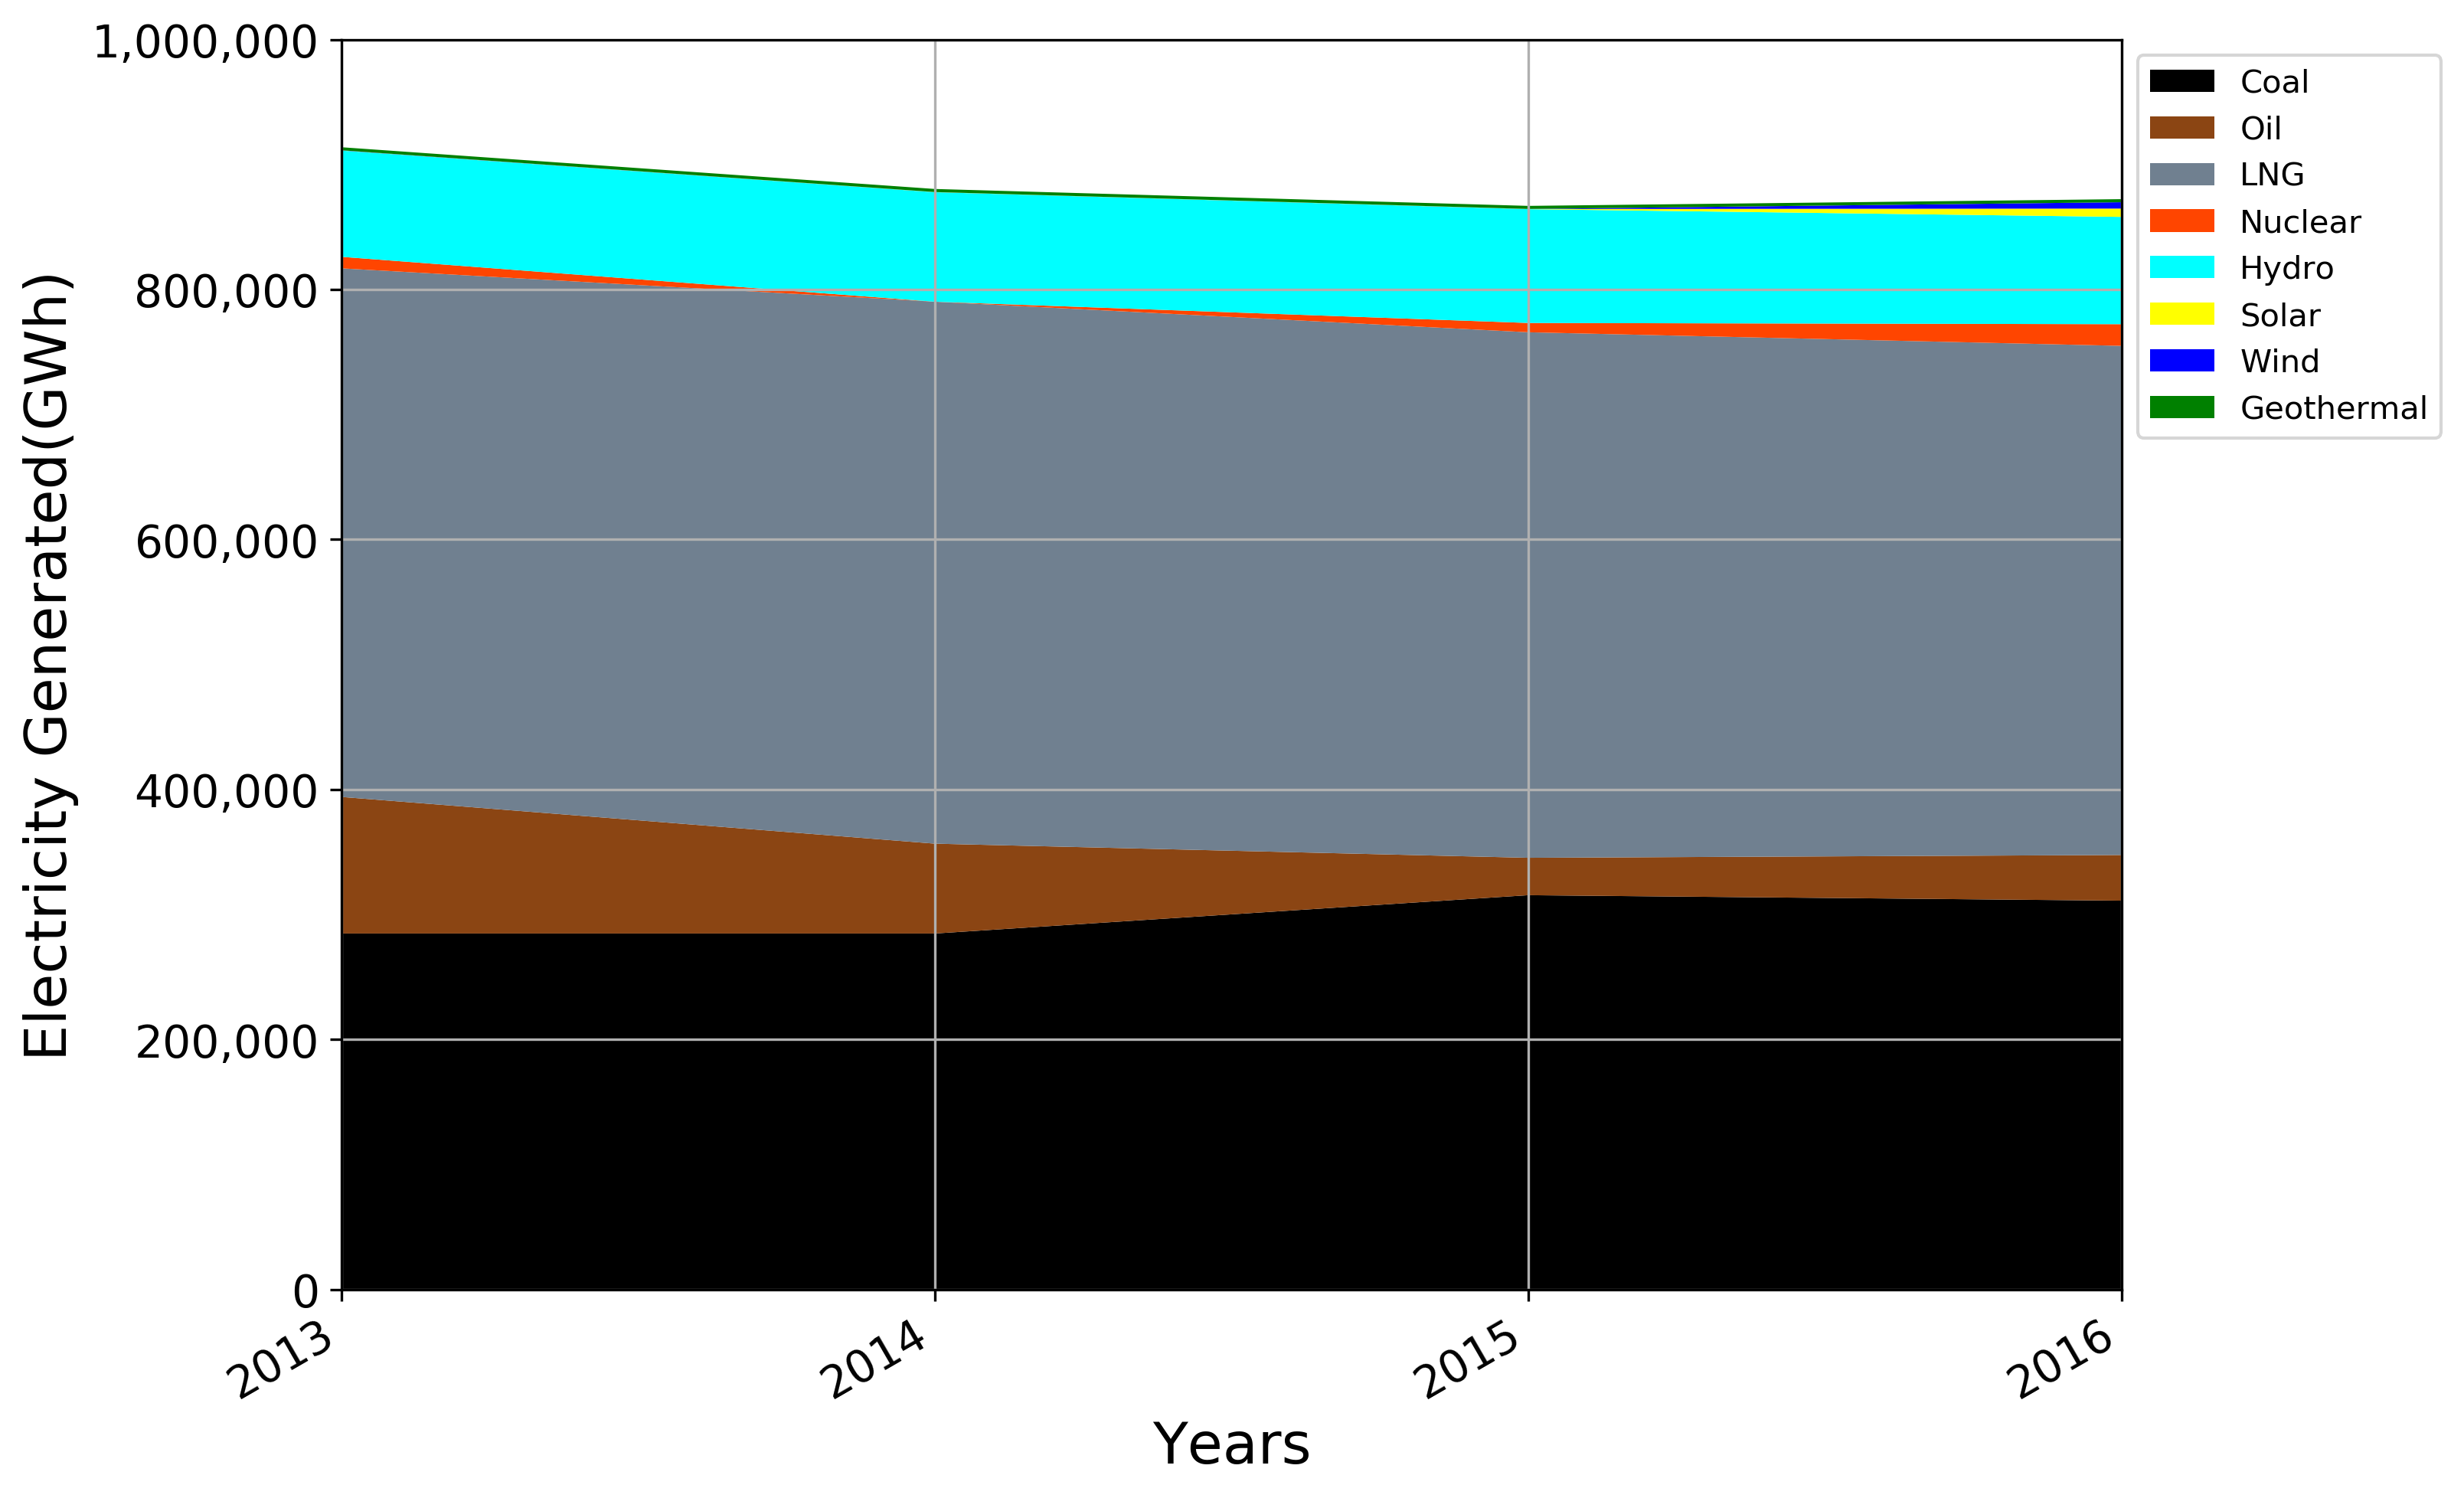
\includegraphics[scale=0.5]{figures/IC}
\caption{Electricity generation that defines the initial condition of the model.}
\end{figure}

\begin{table}[!ht]
	\caption{Initial condition CO$_2$ emissions compared to the model and data from the Carbon Trust.}
	\vspace{0.1in}
	\begin{tabularx}{\textwidth}{p{0.08\textwidth} p{0.35\textwidth} p{0.35\textwidth} p{0.15\textwidth}}
		\hline
\textbf{Year} & \textbf{Model Emissions} & \textbf{Actual Emissions} & \textbf{Error} \\
  & Mt CO$_2$-eq. & Mt CO$_2$-eq. &  \\
\hline
2013 & 603.62 & 592.4 & 1.89 \% \\
2014 & 582.27 & 572.6 & 1.69 \% \\
2015 & 572.53 & 560.3 & 2.18 \% \\
2016 & 565.94 & 552.8 & 2.38 \% \\
\hline 
	\end{tabularx}
\label{ic-co2}
\end{table}
The electricity demand in the near term is expected to increase by 1.7\% per year (cite electricity review). However, in the long run, the demand should eventually plateau, if not decrease altogether, due to the ageing population of Japan. In the absence of long term projections, our model approximates the gradual reduction in the annual demand increase rate, and its eventual reduction to 0\% per year, as shown in table \ref{demand}. The demand increases linearly for all intermediate years.

\begin{table}[!ht]
	\caption{Demand increase over time.}
	\vspace{0.1in}
	\begin{tabularx}{\textwidth}{p{0.5\textwidth} p{0.5\textwidth}}
		\hline
\textbf{Year} & \textbf{Annual demand increase} \\
\hline
2017-2030 & 1.7 \% \\
2031-2050 & 1.0 \% \\
2051-2070 & 0.5 \% \\
2070-2100 & 0.0 \% \\
\hline 
	\end{tabularx}
\label{demand}
\end{table}
The CO$_2$ constraints common to all the models are as shown in table \ref{co2-limits}. The CO$_2$ limit for intervening years is linearly interpolated to ensure gradual transitions. 
\begin{table}[!ht]
	\caption{CO$_2$ constraints.}
	\vspace{0.1in}
	\begin{tabularx}{\textwidth}{p{0.1\textwidth} p{0.5\textwidth}p{0.1\textwidth} p{0.2\textwidth}}
		\hline
\textbf{Year} & \textbf{Absolute Emission limit} & \textbf{Base Year} & \textbf{Reduction from Based Year} \\
\hline
2030 & 438 Mt CO$_2$-eq. & 2013 & 26 \% \\
2050 & 75 Mt CO$_2$-eq. & 1990 & 80 \% \\
2100 & 75 Mt CO$_2$-eq. & 1990 & 80 \% \\
\hline 
	\end{tabularx}
\label{co2-limits}
\end{table}

\subsection{Existing technologies}

For time periods excluding the initial condition, the model can choose to deploy various renewables and base-load electricity generation technologies. The economic data and growth rates for these technologies are defined in tables \ref{existing-eco} and . The capital and \gls{OM} costs of offshore wind are significantly greater due to Japan's unusually deep seabed and the generally underdeveloped wind sector.

\begin{table}[!ht]
	\caption{Economic data for existing technologies.}
	\vspace{0.1in}
	\begin{tabularx}{\textwidth}{p{0.2\textwidth} p{0.16\textwidth} p{0.16\textwidth} p{0.16\textwidth}  p{0.1\textwidth} p{0.1\textwidth}}
		\hline
\textbf{Technology} & \textbf{Investment Cost} & \textbf{Fixed \gls{OM} costs} & \textbf{Variable \gls{OM} costs} & \textbf{Lifetime} & \textbf{Capacity Factor}\\
  & USD/kW & USD/kW & USD/MWh & Years & \\
\hline
Nuclear & 6317 & 121.13 & 2.36 & 60 & 0.90\\
Solar & 1307 (2017) & 15.19 & 0 & 25 & 0.14\\
Onshore Wind & 3454 (2017) & 136.37 & 0 & 25 & 0.4\\
Offshore Wind(Fixed) & 7772.73 & 341 & 0 & 25 & 0.44\\
Offshore Wind(Floating) & 12897 & 423 & 0 & 25 & 0.44\\
Li-ion Storage & 1876 (2017) & 10 & 0.3 & 10 & 4h/24h \\
Natural Gas &  1079 & 14 & 2.54 & 10 & 0.55 \\
\gls{USC} & 3661 & 40.41 & 4.48 & 10 & 0.55 \\
\hline 
\end{tabularx}
\label{existing-eco}
\end{table}

\subsection{Emerging technologies}

\subsection{Base scenarios}
%approach, goal, what are we hoping to learn
\begin{table}[!ht]
	\caption{Scenario definition.}
	\vspace{0.1in}
	\begin{tabularx}{\textwidth}{p{0.33\textwidth} p{0.33\textwidth} p{0.33\textwidth}}
\hline 
\textbf{Scenario}& \textbf{Emerging tech.} & \textbf{New nuclear} \\
                 & \textbf{enabled} & \textbf{enabled} \\
                  \hline
%1               &   \xmark       &      \greencheck     \\ 
%2               & \xmark       &         \xmark       \\ 
%3               &   \greencheck     &      \greencheck     \\ 
%4               &   \greencheck     &         \xmark       \\
1               &   No       &      Yes     \\ 
2               &  No       &         No       \\ 
3               &   Yes     &      Yes     \\ 
4               &   Yes     &         No       \\

\hline
	\end{tabularx}
\label{scen-table}
\end{table}
\subsection{Sensitivity analysis}
%approach, goal, what are we hoping to learn

